\documentclass{article} 

\input{setup/a1.setup.tex}

\addbibresource{references.bib}
\addbibresource{setup/d1.ext_references.bib}

\usepackage{tikz}
\usetikzlibrary{decorations.markings}
\usetikzlibrary{decorations.pathmorphing}
\usetikzlibrary{shapes.geometric}
\tikzset{->-/.style={
		decoration={
			markings,
			mark={at position .5 with {\pgftransformscale{2}\arrow{>}}}
		},
		postaction={decorate}
	}
}
\tikzset{
	square/.style={
		regular polygon,
		regular polygon sides=4,
		minimum size=0.5cm,
		draw
	},
	triangle/.style={
		regular polygon,
		regular polygon sides=3,
		minimum size=0.5cm,scale=0.7,
		draw
	}
}
\tikzstyle{snake it}=[decorate,decoration={snake, #1,}]
\usetikzlibrary{angles,quotes,calc,positioning} % Load the calc library
\usepackage{cancel}
%\bibliography{references.bib}
\DeclareDocumentCommand{\quote}{m}{%
	``#1''%
}
\def\proposed{%
	\color{green!30!black}%
}
\begin{document}
% \setcounter{footnote}{-1}

%%%%%%%%%%%%%%%%%%%%%%%%%%%%%%%%%%%%%%%%%%

\begin{minipage}{0.9\linewidth}
	\centering{\Large\bfseries Travel-Time Tomography and Sound Speed Field Estimation in Water\\
	\large An investigative research on SVD-based inversion, and other advancements}
\end{minipage} \\[0.5cm]
\begin{center}
\begin{minipage}{0.7\linewidth}
	%
		\itshape This text aims to be an investigative research on SVD-based inversion for Sound Speed field estimation in water through the Travel-Time Tomography technique. It also contains other advancements and applications for the standard model (previously described), along with results and comparisons. It is a continuation of the aforementioned \quote{Literature Review and standard model description} document, and assumes its reading.
	\end{minipage}
\end{center}
\section{Sound Speed Field Estimation}

Although the speed of sound $c$ in water is considered constant at around $1500 \si{\meter}/\si{\second}$, it can vary when considering environments of both small and large scales, respectively in small and large proportions \cite{kieffer_sound_1977,trusler_determination_2017,li_sound_2015,pinson_sound_2010}. Many properties can affect the speed of sound in water, such as pressure, temperature, salinity, and water currents \cite{wilson_speed_1959,medwin_fundamentals_1998,mcdougall_getting_2011,delgrosso_new_1974}. As these properties vary over the body of water, so does the velocity, creating a sound speed field (SSF) in the body of water. Although the term sound speed profile \cite{li_acoustic_2019,li_sound_2015,pinson_sound_2010} (SSP) is also commonly used, it usually refers to the $1D$ scenario of estimation.

Initial works in the topic of estimating the velocity field in water aimed at estimating these key properties, as well as the relationship between them and the velocity of water. Works such as \cite{wilson_speed_1959,medwin_fundamentals_1998,mcdougall_getting_2011,delgrosso_new_1974,chen_speed_1977,wong_speed_1995,roquet_accurate_2015} operated under this framework, with some still being used today to model the behavior of water currents on a global scale.

In \cite{wilson_speed_1959}, their experiments showed that (in distilled water) $c$ has a strictly positive relationship with pressure, and a parabolic correlation with temperature. That is, an increase in pressure directly corresponds to an increase in $c$, and similarly with temperature up to a certain point, after which increases in temperature either don't affect $c$, or even cause a decrease in velocity. In \cite{medwin_fundamentals_1998}, empirical models for the $c$ are provided, also taking salinity into account in their formulation.

The TEOS-10 model \cite{mcdougall_getting_2011} is another method for estimating the velocity field given the temperature, pressure, and salinity parameters in the body of water, solving chemical-thermodynamics equations to find the adequate velocity distribution.

The pursuit of knowing the speed of sound at each point of a body of water -- the SSF -- allows the knowledge of the properties of a wave that travels through this medium. By Snell's law, a change in speed of a wave also changes its direction, therefore a wave that travels through a sufficiently large body of water will be also affected within it, resulting in curves, refractions, reflections, and formation/dissolution of beams.

By knowing the SSF, we can know the path a unidirectional wave would course. By treating an omnidirectional wave as a cluster of unidirectional waves, we can calculate the travel-time between the source and any point within the medium, as well as its wavefront's profile.

Most modern SSF estimation approaches avoid estimating these properties, and treat this SSF estimation as an inversion problem. That is, since the knowledge of the SSF allows calculating the path of a wave through the medium, then the knowledge of these paths permits the estimation of the SSF in the medium. Different techniques tackle this inversion problem by using measurements, and employing the acquired information through different lenses.

Most techniques utilize sound sources and receptors within the body of water, and by comparing the properties of the waves that are produced and received, estimate the path of the waves; and from this, the SSF of the water body.

\subsection{Methods for SSF inversion}

Many different methods can be used for estimating the SSF, using different information acquired by sensors along the body of water. These data can be the travel-time between source and receptors, the measured sound pressure, difference in phase and amplitude between the devices, or even the temperature-salinity-pressure used in the previously cited methods. Along with this, the techniques can use these measurements through either direct SSF estimation methods, as well as via machine learning.

\subsubsection{Travel-time tomography}

Travel-time tomography (TTT) \cite{bormann_seismic_2012,stefanov_travel_2019} is one of the simplest methods for SSF estimation. It uses the difference in arrival time of the acoustics signals at the sensors, requiring a spatial distribution of sources and receiver(s) for sufficient spatial resolution.

In general, the SSF is discretized in layers or cells, where each behaves as having a constant sound speed. Then, the wavepath's length in each layer is calculated, resulting in a system of equations that is used to estimate the velocity in each layer. It can also work with assumed functions for the SSF, ditching the layering assumption, but increasing the problem's complexity.

Its simpleness, robustness and computational efficiency are its main advantages, the later allowing real-time implementation. However, it depends on a precise positioning and syncing of the devices, and its discretization assumption results in limited resolution.

\subsubsection{Matched field processing and inversion}
In matched field processing (MFP) \cite{gemba_adaptive_2017} and matched field inversion (MFI) \cite{dosso_bayesian_2011}, the measured pressure data in the receivers is compared to acoustic pressure models for different SSFs, matching and adapting the models to the data through optimization algorithms in order to find the most similar one.

These techniques are similar to beamforming, which are used in many fields such as acoustics and signal processing \cite{schmidt_environmentally_1990,brienzo_broadband_1993}, where both use spatial correlation between the receivers and their measurements, and model the acoustic field through them.

MFP and MFI also employ modal decomposition of the signals, with each mode behaving differently in water. They incorporate more complex information regarding the signals, such as amplitude and phase, depending not only in travel time. Among their advantages, we have a better use of obtained data, enhanced spatial resolution -- compared to TTT -- and improved robustness to noise due to coherent processing. However, it requires spatial-temporal information on the source and receivers, such as directivity and spectral behavior. It also isn't very suitable for very large bodies, given that a larger body would result in an exponentially more complex acoustic pressure model; and is more computationally complex, as well as susceptible to local minima.

\subsubsection{Full waveform inversion}

Full waveform inversion (FWI) techniques \cite{virieux_overview_2009,fichtner_multiscale_2013} aim the waveform reconstruction of the signals present in the SSF, considering many different behaviors that are neglected by the aforementioned techniques. Here, the error between the estimated and measured waveforms is minimized, being implemented in either time- or frequency-domains.

Given this, the FWI technique is among the ones that maximally use the receivers' available data, and resulting in the most faithful SSF, as well as maximally using the available signals. However, due to considering complex signal interactions and multiple wavepaths, there is a significant increase in the mathematical and computational complexity. This, coupled with the non-linearity of the problem, results in a very intense and sometimes unfeasible technique, that also requires a decent initial parameter estimation for its robustness and convergence.
\subsection{Fundamentals of travel-time tomography}

Travel-time tomography (TTT) \cite{bormann_seismic_2012,stefanov_travel_2019} is one of the simplest methods for SSF estimation. It uses the difference in arrival time of the acoustics signals at the sensors, requiring a spatial distribution of sources and receiver(s) for sufficient spatial resolution.

In general, the SSF is discretized in layers or cells, where each behaves as having a constant sound speed. Then, the wavepath's length in each layer is calculated, resulting in a system of equations that is used to estimate the velocity in each layer. It can also work with assumed functions for the SSF, ditching the layering assumption, but increasing the problem's complexity.

Its simpleness, robustness and computational efficiency are its main advantages, the later allowing real-time implementation. However, it depends on a precise positioning and syncing of the devices, and its discretization assumption results in limited resolution.

\begin{figure}[H]
	\centering
	\begin{tikzpicture}[scale=1.5]
		\coordinate (tl) at (-3, 2);
		\coordinate (tr) at (3, 2);
		\coordinate (bl) at (-3, -2);
		\coordinate (br) at (3, -2);
		\coordinate (cc) at (0,0);
		\coordinate (tc) at (0,2);
		\coordinate (bc) at (0,-2);
		\coordinate (cl) at (-3, 0);
		\coordinate (cr) at (3,0);
		\coordinate (source) at ($(bl)!0.95!(br)$);
		\coordinate (receiver) at ($(bl)!0.9!(tl)$);
		\draw[gray,fill=none] (tl) rectangle (br);
		\draw[->-,thick] (source) to[out=120,in=-18] (receiver) node[pos=0.5,anchor=center,black] {$\bvr[v]$};
		%		\filldraw[blue!50!black] (receiver) rectangle (2,2);
		%		\filldraw[green!50!black] (source) circle (3pt);
		\node[square,fill=blue!70!black] () at (receiver) {};
		\node[triangle,fill=green!70!black] () at (source) {};
		
	\end{tikzpicture}
	\caption{Wave path on heterogeneous and continuously variable environment.}
	\label{fig:sec2:wavepath_heterogeneous-variable_environment}
\end{figure}

Consider a wave that follows the path from \cref{fig:sec2:wavepath_heterogeneous-variable_environment}, this being represented by the curve $\bvr[v]$. Assuming that the speed of sound $c(\bvp)$ is a function of space ($\bvp = [x,y,z]$), then the travel time along the curve $\bvr[v]$ is
\begin{equation}
	t_{\bvr[v]} = \int_{\bvr[v]} \frac{1}{c(\bvp)} \dd\bvp.
\end{equation}

The objective is to, given a set of $N$ measures $t_{\bvr[v]{i}}$, these representing different wave paths, estimate the sound speed field $c(\bvp)$.

Different approaches can be taken to solve this problem, including to discretize space, approximate the SSF as polynomial through Spline or least-squares fitting, among others. This technique can also be employed in 1D, 2D or 3D situations, and acquiring spatial diversity through either (or both) multi-source or multi-receiver means.

Most models estimate the slowness (inverse of speed) field. Note that SSF can both mean \quote{sound speed field} and \quote{sound slowness field}. Since both quantities are the reciprocal of one another, the SSF acronym will be indiscreetly used for both.

\subsection{Standard discrete travel-time tomography approach}
\label{subsec:sec2:standard_ttt_approach}

All of the cited papers took an approach similar to the one established below. Differences may arise from ignoring ray bending, type of regularization in the minimization process, amount and positioning of sources and receivers, final purpose for the TTT, or some other particularization or assumption.

In these regards, the most complete papers are the ones by Ali \cite{ali_opensource_2019}, Phillips \cite{phillips_traveltime_1991}, and Hormati \cite{hormati_robust_2010}, where they consider regularization, ray bending, and a large amount of sources and receivers. We now will lay the common ground among all the presented papers, the median modeling considerations and formulations, as well as some important distinctions and particularities that are shared between some of them. Note that the framework presented here isn't identical to the ones in the cited papers \cite{aki_determination_1977,aki_determination_1976,ali_opensource_2019,hormati_robust_2010,jeong_investigating_2024,hellmann_borehole_2023,phillips_traveltime_1991,zhang_nonlinear_1998,dines_computerized_1979}, and only highlights the similarities and mostly-shared ground between them.

Let's assume the environment to be modeled is divided into an $\sz{N_1}{N_2}$ grid of cells (horizontal $\mtimes$ vertical), with a total of $N = N_1\cdot N_2$ cells. A total of $M$ rays are produced, between any number of sources and receivers. We denote $\bvs \in \re^{\sz{N}{1}}$ positive vector representing the slowness in each cell, and $\bvR{m}(\bvs) \in \re^{\sz{N}{1}}$ vector containing the length traversed in each cell, by the $m$-th ray. The length-vector $\bvR{m}(\bvs)$ is commonly obtained externally via a fast-marching algorithm or another solver for the Eikonal equation, considering Fermat's principle of least time, and Snell's law $\bvR{m}(\bvs)$. $\bvR{m}(\bvs)$ can also be obtained directly if one considers an SSF with small perturbations, where ray-bending effects can be ignored, and the path is assumed linear between source and receiver. With this, the travel-time for the $m$-th ray is $t_m$, being given by
\begin{equation}
	t_m(\bvs) = \tr{\bvr{m}}(\bvs) \bvs
\end{equation}

Now we let $\bvt(\bvs) \in \re^{\sz{M}{1}}$ vector of travel-times for the current model, for all $M$ considered rays; and $\bvR(\bvs) \in \re^{\sz{M}{N}}$ matrix, where the $m$-th row is $\tr{j_m}(\bvs)$. With this, our minimization problem becomes minimizing the error $E(\bvs)$, this being translated into
\begin{equation}
	\opt{\bvs} = \arg\min_{\bvs} E(\bvs) = \norm{\bvR(\bvs) \bvs - \bvt{\obs}}^2
	\label{eq:sec2:def_minimization_bvz}
\end{equation}
where $\bvt{\obs}$ is the observed travel-time for each ray.

Note that this problem is non-linear and recursive: the solution to the ray paths, given by $\bvR(\bvs)$, depends on the slowness field $\bvs$. Meanwhile, the field model depends on the achieved solution for the ray paths, $\bvR(\bvs)$. Given the non-linearity of the problem, this search is usually done iteratively, following
\begin{subequations}
	\begin{gather}
		\bvs{i+1} = \arg\min_{\bvs{i+1}} E(\bvs{i+1}) = \norm{\bvR(\bvs{i}) \bvs{i+1} - \bvt{\obs}}^2 
		\label{subeq:sec2:iterative_minimization:eq1}\\
		\nabla E(\bvs{i+1}) = 2\tr{\bvR}(\bvs{i}) \pts{\bvR(\bvs{i}) \bvs{i+1} - \bvt{\obs}}
		\label{subeq:sec2:iterative_minimization:eq2}
	\end{gather}
	\label{eqs:sec2:iterative_minimization}
\end{subequations}

Usually, this problem is ill-posed, and requires extra conditions for a unique solution. The most common is regularization, which leads to the problem
\begin{subequations}
	\begin{gather}
		\bvs{i+1} = \arg\min_{\bvs{i+1}} E(\bvs{i+1}) = \norm{\bvR{i} \bvs{i+1} - \bvt{\obs}}^2 + P_\alpha(\bvs{i+1})\\
		\nabla E(\bvs{i+1}) = 2\bvR[T]{i} \pts{\bvR{i} \bvs{i+1} - \bvt{\obs}} + \nabla P_{\alpha}(\bvs{i+1})
	\end{gather}
	\label{eqs:sec2:iterative_minimization_Ezi}
\end{subequations}
with $\alpha$ being a controlling parameter; and, assuming that the regularization function can be given by $P_{\alpha}(\bvs{i+1}) = \alpha^2\norm{\bvD\bvs{i+1}}^2$ where $\bvD$ is a square matrix, its solution is
\begin{equation}
	\bvG{i} = \inv*{\tr{\bvR{i}} \bvR{i} + \alpha^2 \tr{\bvD}\bvD} \bvR[T]{i}
	\label{eq:sec2:solution_regularization-problem_simple}
\end{equation}
for this inversion step to be possible, it is sufficient that $\bvD$ is a full-rank matrix\footnote{\label{footnote:positive-definite_inversion}By definition, $\bvR[T]{i} \bvR{i}$ is positive-semidefinite, $\tr{\bvD}\bvD$ is positive-definite if it is full-rank square matrix, and the sum of a positive-semidefinite and a positive-definite is always positive-definite, this being a sufficient condition for invertibility.}.

The regularization matrix $\bvD$ can be chosen to improve a range of metrics. Choosing $\bvD = \Id$ \cite{phillips_traveltime_1991} results in the minimization also considering the root mean-square (RMS) of the slowness vector; this is equivalent to considering the presence in white noise in the measurements, and trading model accurateness for noise rejection. Choosing $\bvD z \approx \nabla^2 s(x,y)$, (discretely) approximating the Laplacian of the (continuous) slowness field \cite{zhang_nonlinear_1998,ali_opensource_2019}, resulting in a minimization that penalizes the Laplacian of the achieved slowness field; that is, a solution that also considers the curvature/jumps in the SSF, searching for a smoother field.

Another interesting tool that is seen in the literature \cite{phillips_traveltime_1991,meyerholtz_convolutional_1989} is to employ a blur on the gradient. That is, we define that
\begin{equation}
	E(\bvs{i+1}) = \norm{\bvR[d]{i} \bvs[d]{i+1} - \bvt{\obs}}^2 + P_\alpha(\bvs[d]{i+1})
\end{equation}
where $\bvR[d]{i} = \bvR{i}\bvB{i}$ and $\bvs[d]{i+1} = \inv{\bvB{i}} \bvs{i+1}$, and $\bvB{i}$ is the $i$-th iteration's blurring matrix (this being based on a Gaussian blur, or any other averaging kernel, that decreases in radius at each iteration). In this scenario, the solution $\bvs{i+1}$ is
\begin{equation}
	\bvG{i} = \bvB{i} \inv*{\tr{\bvB{i}} \tr{\bvR{i}} \bvR{i} \bvB{i} + \alpha^2 \tr{\bvD}\bvD} \tr{\bvB{i}} \bvR[T]{i}
\end{equation}

To achieve this, the regularization function has to be adapted, such that $P_{\alpha}(\bvs{i+1}) = \alpha^2 \norm{\bvD \inv{\bvB{i}} \bvs{i+1}}^2$; this means the regularization is applied on the ``reverse blurred'' signal. As stated, the blurring matrix $\bvB{i}$ depends on the iterator $i$. Usually, the blur radius is decreased for increasing $i$, aiming at gradually finding a more refined and accurate (less blurry) solution.

This convolutional averaging (also called ray broadening \cite{meyerholtz_convolutional_1989,phillips_traveltime_1991}) can help find solutions by scattering the rays and expanding the paths taken to neighboring cells, thus dealing with the problem of some cells not being traversed by any rays.
{\proposed
\section{SVD pseudo-inversion}

\textit{\small This section is one for a proposed method, suitable for situations of rank-deficient ill-posed problems. Although in this literature review, it covers the implementation of a novel technique within the context of travel-time tomography.}

Given the inverse step necessary in the ill-posed problem, one possibility for addressing this hurdle -- as briefly commented in \cref{subsubsec:rank-definicient-minimization} -- is the use of an SVD-based pseudo-inversion, for situations where $\bvJ{i}$ is rank-deficient. 

Given $\bvJ{i}$, we write it through its singular value decomposition, as
\begin{equation}
	\bvJ{i} = \bvU \bvSi \bvV[T]
\end{equation}
in which $\bvU \in \re^{\sz{M}{M}}$ and $\bvV \in \re^{\sz{N}{N}}$ are the left- and right-singular vectors of $\bvJ{i}$, forming and orthonormal bases; and $\bvSi \in \re^{\sz{M}{N}}$ is a diagonal matrix, given by
\begin{equation}
	\bvSi = \begin{bmatrix}
		\lambda_1 & 0 & \cdots & 0 \\
		0 & \lambda_2 & \cdots & 0 \\
		\vdots & \vdots & \ddots & \vdots \\
		0 & 0 & \cdots & \lambda_N \\
		0 & 0 & \cdots & 0 \\
		\vdots & \vdots & \ddots & \vdots \\
		0 & 0 & \cdots & 0
	\end{bmatrix}
\end{equation}
with $\lambda_1 \geq \lambda_2 \geq \cdots \geq \lambda_N$ being the singular values of $\bvJ{i}$, in decreasing order. Given the properties of the SVD process, all these singular values are strictly non-negative. By definition, $\bvU \equiv \bvU{i}$ (similarly for $\bvSi$ and $\bvV$), although this relation was omitted for clarity of notation.

\subsection{SVD pseudo-inverse}

Assuming that $\rank{\bvJ{i}} = R < N$, then $\lambda_{R+1} = \cdots = \lambda_{N} = 0$. In this scenario, $\pinv{[\bvJ[T]{i} \bvJ{i}]}$ -- where $\pinv*{\cdot}$ denotes the pseudo-inverse -- can be obtained as
\begin{equation}
	\begin{split}
		\pinv*{\bvJ[T]{i} \bvJ{i}}
		& = \pinv*{\bvV \bvSi[T] \bvU[T] \bvU \bvSi \bvV[T]} \\
		& = \pinv*{\bvV \bvSi[T] \bvSi \bvV[T]} \\
		& = \bvV \pinv*{\bvSi[T] \bvSi} \bvV[T] \\
		& = \bvV \pinv{\bvSi} \pinv{{\bvSi[T]}} \bvV[T]
	\end{split}
\end{equation}
where the orthogonality of $\bvV$ and the distributive property of the pseudo-inverse (considering the orthogonality of $\bvV$ and of the columns of $\bvSi$) were used; and $\pinv{\bvSi} \in\re^{\sz{N}{M}}$ is a diagonal matrix, with its entries being the reciprocal of the singular values of $\bvJ{i}$. Additionally, $\pinv{\bvSi}$ can be explicitly written as
\begin{equation}
	\pinv{\bvSi} = \begin{bmatrix}
		\inv{\lambda_1} & 0 				& \cdots & 0 				& 0 	 & \cdots & 0 \\
		0 				& \inv{\lambda_2} 	& \cdots & 0 				& 0 	 & \cdots & 0 \\
		\vdots 			& \vdots 			& \ddots & \vdots 			& \vdots & \ddots & \vdots \\
		0 				& 0 				& \cdots & \inv{\lambda_R}	& 0 	 & \cdots & 0 \\
		0				& 0					& \cdots & 0 				& 0		 & \cdots & 0 \\
		\vdots 			& \vdots 			& \ddots & \vdots 			& \vdots & \ddots & \vdots \\
		0				& 0					& \cdots & 0 				& 0		 & \cdots & 0
	\end{bmatrix}_{\sz{N}{M}}
\end{equation}
in which the last $M-R$ columns, and last $N-R$ rows, are strictly $0$. With this pseudo-inversion of $\pinv{\bvSi}$, and therefore of $\bvJ[T]{i} \bvJ{i}$, the solution to the minimization problem is
\begin{equation}
	\begin{split}
		\bvG{i}
		& = \pinv*{\bvJ[T]{i} \bvJ{i}} \bvJ[T]{i} \\
		& = \bvV \pinv{\bvSi} \pinv{{\bvSi[T]}} \bvV[T] \bvV \bvSi[T] \bvU[T] \\
		& = \bvV \pinv{\bvSi} \bvU[T]
	\end{split}
	\label{eq:sec2:solution-G_pseudo-inverse}
\end{equation}
where, by definition of the pseudo-inverse, $\pinv{\bvSi} \pinv{{\bvSi[T]}} \bvSi[T] = \pinv{\bvSi}$. Via properties of the pseudo-inverse, we also have that
\begin{equation}
	\bvG{i} = \pinv{\bvJ{i}}
\end{equation}
Although this formulation is completely valid, it will not be used going forward, as making explicit the SVD form of $\pinv{\bvj{i}}$ can be advantageous, in the algebraic steps.

In the particular case where $R = N$, this implies that $\bvJ[T]{i} \bvJ{i}$ is positive-definite, thus full-rank and straightforwardly invertible. Therefore, the pseudo-inverse isn't necessary in this particular scenario. However, as the pseudo-generalizes the inverse in this case, its application can be useful to highlight and expose properties of the treated problem.

\subsection{Cost function and gradient with SVD}

The gradient for $\bvz{i+1} = \bvV \pinv{\bvSi} \bvU[T] \bvt$ is
\begin{equation}
	\begin{split}
		\nabla E(\bvz{i+1})
		& = 2\pts{\bvV \bvSi[T] \bvU[T] \bvU \bvSi \bvV[T] \bvV \pinv{\bvSi} \bvU[T] \bvt - \bvV \bvSi[T] \bvU[T] \bvt} \\
		& = 2\pts{\bvV \bvSi[T] \bvSi \pinv{\bvSi} \bvU[T] \bvt - \bvV \bvSi[T] \bvU[T] \bvt} \\
		& = 2\pts{\bvV \bvSi[T] \bts{\Id{M;R} - \Id{M}} \bvU[T] \bvt}
	\end{split}
\end{equation}
where $\Id{M;R} \in \re^{\sz{M}{M}}$ is a diagonal matrix with the first $R$ entries being $1$, and the remaining $M-R$ ones being $0$; and $\Id{M} \in \re^{\sz{M}{M}}$ is the identity matrix. From this, $\Id{M;R} - \Id{M}$ has its first $R$ diagonal entries $0$, and the last ones $-1$. Since all rows of $\bvSi[T]$ are in the null space of $\Id{M;R} - \Id{M}$ (only the first $R$ entries of any row of $\bvSi[T]$ are non-zero, exactly where $\Id{M;R} - \Id{M}$ is zero), then $\bvSi[T]\bts{\Id{M;R} - \Id{M}} = \bv0$. Therefore,
\begin{equation}
	\begin{split}
		\nabla E(\bvV \pinv{\bvSi} \bvU[T] \bvt)
		& = 2\pts{\bvV \,\bv0\, \bvU[T] \bvt} \\
		& = \bv0
	\end{split}
\end{equation}

This verification ensures that $\bvz{i+1} = \bvV \pinv{\bvSi} \bvU[T] \bvt$ is a solution to the minimization process from \cref{eqs:sec2:iterative_minimization_Ezi}.

We denote $\bvU{k}$ as the first $k$ columns of $\bvU$, $\bvU{-k}$ as the last $k+1$ columns of $\bvU$, and $\bvU{(j\sim k)}$ as the columns from $j$ to $k$ (inclusive) of $\bvU$. Using this, the cost function can be explicitly obtained, being given by
\begin{equation}
	E(\bvz{i+1}) = \bvt[T] \bvU{-R} \bvU[T]{-R} \bvt
\end{equation}

\subsection{Null-space exploitation}

We can expand on the solution $\bvz{i+1} = \bvV \pinv{\bvSi} \bvU[T] \bvt$ by exploiting the null space of $\bvJ{i}$. We write
\begin{equation}
	\bvV = \left[\begin{array}{c|c}
		\!\bvV{1} & \bvV{2}\!
	\end{array}\right]
\end{equation}
where $\bvV{1}\in \re^{\sz{N}{R}}$ are the first $R$ columns of $\bvV$, $\bvV{2} \in \re^{\sz{N}{(N-R)}}$ the remaining $N-R$ columns of $\bvV$, and $[\cdot|\cdot]$ denotes matrix concatenation. Note that $\bvV{2}$ is relative to last $N-R$ zero rows of $\bvSi$, which are strictly $0$; this implies that the columns of $\bvV{2}$ form an orthonormal basis for the null space of $\bvJ{i}$.

Given a coordinate vector $\bvmu \in \re^{\sz{(N-R)}{1}}$, any $\bvz[b] = \bvV{2} \bvmu$ will be within the null space of $\bvSi$, and therefore $\bvJ \bvz[b] = \bvU \bvSi \bvV[T] \bvV{2} \bvmu$ will be by definition $\bv0$. This means that, for $\bvz{i+1} \equiv \bvz{i+1}(\bvmu) = \bvV \pinv{\bvSi} \bvU[T] \bvt + \bvV{2} \bvmu$, we have
\begin{subequations}
	\begin{gather}
		\nabla E(\bvV \pinv{\bvSi} \bvU[T] \bvt + \bvV{2} \bvmu) = \bv0, \\
		E(\bvV \pinv{\bvSi} \bvU[T] \bvt + \bvV{2} \bvmu) = E(\bvV \pinv{\bvSi} \bvU[T] \bvt)
	\end{gather}
\end{subequations}

\subsection{Secondary metric minimization}

Given another metric, this information on $\bvmu$ can be leveraged to find an optimal solution within this metric, while keeping to $\nabla E(\bvz{i+1}) = \bv0$. For example, we can define a new cost function $F(\bvmu)$, given by
\begin{equation}
	F(\bvmu) = \norm{\bvD \pts{\bvV \pinv{\bvSi} \bvU[T] \bvt + \bvV{2}\bvmu}}^2
\end{equation}
where $\bvD$ is a matrix that governs this secondary metric. For example, we take $\bvD$ to be the previously determined discrete approximation for the Laplacian. Given that the column-orthogonality of $\bvV{2}$ implies $\rank{\bvV{2}} = N-R$, and assuming that $\bvD$ is a full-rank matrix, a solution to this problem can be directly found, as
\begin{equation}
	\bvmu = -\inv*{\bvV[T]{2} \bvD[T] \bvD\bvV{2}} \bvV[T]{2} \bvD[T] \bvD \bvV \pinv{\bvSi} \bvU[T] \bvt
\end{equation}

Via properties of the pseudo-inverse, this can be written as
\begin{equation}
	\bvmu = -\pinv*{\bvD \bvV{2}} \bvD \bvV \pinv{\bvSi} \bvU[T] \bvt
	\label{eq:sec2:definition_mu_full}
\end{equation}
With this, the full solution to both minimization problems is given by
\begin{equation}
	\begin{split}
		\bvz{i+1}
		& = \bvV \pinv{\bvSi} \bvU[T] \bvt - \bvV{2} \pinv*{\bvD \bvV{2}} \bvD \bvV \pinv{\bvSi} \bvU[T] \bvt \\
		& = \pts{\Id{N} - \bvV{2} \pinv*{\bvD \bvV{2}} \bvD} \bvV \pinv{\bvSi} \bvU[T] \bvt
	\end{split}
	\label{eq:sec2:definition_zi+1_with_mu}
\end{equation}

This solution both has zero gradient in the error function, and has minimum Laplacian within the space of minimum-error solutions. The main insight for this expansion on $\bvmu$ is, by exploiting the null-space of $\bvJ$, to minimize the primary objective within the row space, and to minimize the second objective within the null space. Note that this procedure only works if $\rank{\bvJ{i}} = R < N$. If $R = N$, there is no null space to be exploited, and the second minimization can't be performed.

Another important remark in this scenario is that $\bvV{2} \pinv*{\bvD \bvV{2}} \bvD$ cannot be simplified. This would require that $\bvV{2}$ has linearly independent rows, which it can't given that $M > N-R$. Another important factor is that the gradient of $F(\bvmu)$ is taken with respect to $\mu$. This implies that within the subspace defined by $\bvV{2}$, the found $\bvmu$ is optimal, but by taking the gradient with respect to $\bvV \pinv{\bvSi} \bvU[T] \bvt$, this gradient will not be $\bv0$.

\subsection{SVD truncation}

Another possibility is to truncate $\bvSi$, or to set an arbitrary number of the smallest diagonal entries of $\bvSi$ to zero. This procedure simultaneously: reduces the effective condition number (ratio between largest and smallest non-zero singular values), improving stability in the inversion problem of minimizing the primary metric; increases the practical null-space of $\bvSi$, allowing for the secondary metric -- here, the Laplacian -- to be more aggressively minimized; but in contrast, introduces some error in the primary minimization, with the minimum found not having truly zero gradient.

We denote $\bvSi[t]{\tilde{R}}$ as a truncated $\bvSi$ with only its first $\tilde{R}$ diagonal entries non-zero; that is, $N-\tilde{R}$ of its diagonal entries are zero, and $R-\tilde{R}$ were forced to zero in the approximation. Trivially, $\tilde{R} \leq R$ for this to be valid. Given this truncation, it is easy to verify that
\begin{equation}
	\begin{split}
		\bvG(\bvz[t]{i}) & \approx \bvG[t](\bvz[t]{i}) \\
		& = \bvV \pinv{\bvSi[t]{\tilde{R}}} \bvU[T]
	\end{split}
\end{equation}
is the optimal solution for the minimization problem with $\bvSi[t]{\tilde{R}}$. The gradient for a solution using this $\bvG[t]{i}$ is
\begin{equation}
	\begin{split}
		\nabla E(\bvz{i+1})
		& = 2\pts{\bvV \bvSi[T] \bvU[T] \bvU \bvSi \bvV[T] \bvV \pinv{\bvSi[t]} \bvU[T] \bvt - \bvV \bvSi[T] \bvU[T] \bvt} \\
		& = 2\pts{\bvV \bvSi[T] \bvSi \pinv{\bvSi[t]} \bvU[T] \bvt - \bvV \bvSi[T] \bvU[T] \bvt} \\
		& = 2\pts{\bvV \bvSi[T] \bts{\Id{M;\tilde{R}} - \Id{M}} \bvU[T] \bvt} \\
		& = 2\pts{\sum_{i=\tilde{R}+1}^{R} \sigma_i \bvv{i} \bvu[T]{i}} \bvt
	\end{split}
\end{equation}
where $\bvv{i}$ and $\bvu{i}$ are the $i$-th row of $\bvV$ and $\bvU$ respectively, and $\sigma_i$ is the $i$-th diagonal element of $\bvSi$. The smaller the entries of $\bvSi$ that were set to zero ($\sigma_i$ for $i \in [\tilde{R}+1,~R]$), the smaller the gradient, and the closer the obtained solution would be to the space of optimal ($\nabla E = 0$) solutions.

We highlight that $\bvSi[t] \bvV[T] \bvV{2} \bvmu$ is still a zero matrix, given that $\bvV[T]{1} \bvV{2} = \bv0$ and $\pts{\bvV[T]{2} \bvV{2}} \in \nul{\bvSi} \subseteq \nul{\bvSi[t]}$. With this, \cref{eq:sec2:definition_mu_full,eq:sec2:definition_zi+1_with_mu} still hold, except for ${\bvSi}$ being replaced by ${\bvSi[t]}$; and the properties of $\bvmu$ not affecting neither cost function nor gradient maintain their validity.

With the previous formulation, the cost function with the truncated SVD will be
\begin{equation}
	E(\bvz[t]{i+1}) = \bvt[T] \bvU{-\tilde{R}} \bvU[T]{-\tilde{R}} \bvt
\end{equation}
or yet, the change in the cost function, compared to that with no truncated singular values, is given by
\begin{equation}
	\Delta E(\bvz[t]{i+1}) = \bvt[T]  \bvU{\tilde{R}\sim R} \bvU[T]{\tilde{R}\sim R} \bvt
\end{equation}
where the columns of $\bvU{\tilde{R} \sim R}$ are exactly the columns of the truncated singular values.

Note that this error is independent of the truncated singular values. Therefore, the choice of $\lambda$'s to truncate isn't related to the increase in the cost function.

\subsection{Spatial super-sampling}

On all previous discussion, it was assumed that $M$ (the number of measurements) is greater than $N$ (the number of discrete cells). However, this requires a large distribution of devices, which isn't necessarily practically feasible.

Since the proposed SVD approach generalizes the traditional inverse (as the scenario where $R = N$ can also be solved using SVD), its use will be continued in this case.

In a scenario where $M < N$, the product $\bvJ[T]{i} \bvJ{i}$ has at most rank $M$, and with it being an $\sz{N}{N}$ matrix, it is guaranteed to be non-invertible. For the previous techniques, this forces the use of a regularization matrix, or the use of non-inverting zero-gradient solvers. For the proposed SVD-based inversion, this just ensures that at least $N-M$ columns of $\bvV$ are within the basis for $\bvJ{i}$'s null-space, guaranteeing the existence of a minimization on $\mu$ and the proposed null-space exploiting step.
}
\newpage

\input{parts/4.Sims.tex}
%\setcounter{section}{5}
\section{Situation-aware modeling}

Although the previous simulations were important to compare the two techniques, showing that their performance is almost identical in both tested scenarios, appropriate results are still necessary in practical situations. In these, the following considerations are taken:
\begin{itemize}
	\item The OBNs positioned at the ocean floor act as sources, and a vehicle (either a ROV or a streamer) that traverses near the surface acts as a receiver;
	\item Vertically sensing the environment with ROVs isn't financially, and should be avoided;
	\item The speed of sound behaves linearly below the SOFAR channel, being feasible to model it by its depth with reasonable accuracy.
\end{itemize}

{
	\begin{figure}[!ht]
	\centering
	\begin{minipage}{0.6\linewidth}
		\centering
		\begin{tikzpicture}
			\begin{heatmap}{\ncols}[newhm,colorbar=false][fill opacity=0.5]
				\addplot3[surf, mesh/cols={\ncols}, mesh/rows={\nrows}, opacity=0.5, draw opacity=0] table[x=x, y=y, z=val, col sep=comma] {figures/data/h71e8/field_observed.csv};
				
				
				\draw[thin, dash pattern = {on 4pt off 1pt}] (axis cs:\pgfkeysvalueof{/pgfplots/xmin},500) -- (axis cs:\pgfkeysvalueof{/pgfplots/xmax},500);
				
				\draw[thin, dash pattern = {on 4pt off 1pt}] (axis cs:\pgfkeysvalueof{/pgfplots/xmin},1000) -- (axis cs:\pgfkeysvalueof{/pgfplots/xmax},1000);
				
				\addplot[forget plot] coordinates {(1850, 150)} node {A};
				\addplot[forget plot] coordinates {(1850, 650)} node {B};
				\addplot[forget plot] coordinates {(1850, 1150)} node {C};
				%
%				{
%					\def\sympath{h298e}
%					\addplot[only marks, mark=o, gray, line width=3pt, mark size=0.5em+0.4pt] table [x=x_pos, y=y_pos, col sep=comma] {figures/data/\sympath/pos_receivers.csv};
%					\addplot[only marks, mark=o, yellow!90!black, very thick, mark size=0.5em+0.4pt] table [x=x_pos, y=y_pos, col sep=comma] {figures/data/\sympath/pos_receivers.csv};
%				}
%				%
%				{
%					\def\sympath{h386f}
%					\addplot[only marks, mark=x, white, line width=2.8pt, mark size=0.5em+0.8pt] table [x=x_pos, y=y_pos, col sep=comma] {figures/data/\sympath/pos_receivers.csv};
%					\addplot[only marks, mark=x, red!50!black, very thick, mark size=0.5em] table [x=x_pos, y=y_pos, col sep=comma] {figures/data/\sympath/pos_receivers.csv};
%				}
			\end{heatmap}
		\end{tikzpicture}
		\colorbar{velocityHeatmap}
	\end{minipage}
	\caption{Modelo em camadas, com camadas A, B, e C.}
	\label{fig:sec5:layered_model}
\end{figure}
}

In practice, both the vehicle and the OBNs act as sources and receivers, with the measurements being done over time for different vehicle positions, assessing the travel-time between the vehicle communicating with the OBN, this processing the commands, and responding. For simplicity, we treat different measurements as occurring simultaneously (assuming the environment's behavior is sufficiently stationary in time), and that the wave travel is only one-way. Also from the considerations, we assume that the receivers can be placed freely up to a $500\si{\meter}$ depth. This leads to a model as in \cref{fig:sec5:layered_model}, where there are 3 layers: A ($0-500\si{\meter}$), B ($500-1000\si{\meter}$), and C ($1000\si{\meter}-\text{floor}$). Notably, layer A is the one where the vehicles traverse, taking measurements, and layer C is the one that can be modeled \textit{a priori}, with its model being refined in the optimization.

Given that the previous results show that both the literature and the proposed approaches are almost identical, the literature one will be chosen, given its more simple mathematical formulation. This, together with the consideration of feasibly modeling the sound speed below a certain threshold, leads to
\begin{equation}
	E(\bvs) = \norm{\bvR \bvs - \bvt{\obs}}^2 + \alpha^2 \norm{\bvD \bvs}^2 + \beta^2 \norm{\calI\pts{\bvs - \bvs{\obs}}}^2
\end{equation}
in which $\alpha$ and $\beta$ are regularization parameters; $\calI$ denotes an $\sz{N}{N}$ diagonal matrix, with its $i$-th element being $1$ if its corresponding cell (element of $\bvs$) is in the C layer, and $0$ otherwise; and $\bvs{\obs}$ is a model for the expected sound speed, only being relevant in the C layer. From the literature approach, the solution to this problem is
\begin{equation}
	{\bvs{i+1}} = \inv*{\bvR[T]{i} \bvR{i} + \alpha^2 \bvD[T] \bvD + \beta^2 \tr{\calI} \calI} \pts{\bvR[T]{i} \bvt{\obs} + \beta^2 \tr{\calI}\calI \bvs{\obs}}
\end{equation}

Note that only the $\bvR{i}$ term depends on the previous $\bvs{i}$ iteration, with the others being either model constants ($\bvD$ and $\calI$), measurement constants ($\bvt{\obs}$ is obtained from the surveys, and $\bvs{\obs}$ from known environmental data), and adjustable parameters ($\alpha$ and $\beta$). A larger $\alpha$ will favor a less varying environment, trading accuracy for smoothness; and a larger $\beta$ will push for a slowness profile that is closer to the model $\bvs{\obs}$.

Another possibility is for $\calI$ to more smoothly transition between the modeled (C) and non-modeled (A and B) layers. For example, it can be $0$ for cells at a depth of up to $900\si{\meter}$, $1$ below $1100\si{\meter}$, and have a transition step between these two depths. For now, we will take the discontinuous approach, switching at the $1\si{\kilo\meter}$ depth.
%\section{Weighted minimization}

In previously presented methods, it is assumed that all measurements are equally important. However, this may not be the case. As an example, consider that some of the measurements were taken when the body of water was being disturbed by heavy water currents, affecting the position of the sensors and the perceived sound speed in water. These measurements are useful, but their data is knowingly less accurate and reliable than that of other measurements, and therefore a weighting step for these measurements can be taken.

Mathematically, this is modeled by adapting \cref{subeq:sec2:iterative_minimization:eq1}. This equation can be expanded, and written as
\begin{equation}
	\bvz{i+1} = \arg \min_{\bvz} \sum_{i=1}^{M} \pts{\bvj[T]{m;i} \bvz - t_{m;\obs}}^2
\end{equation}
in which $\bvj{m;i}$ is the distance traversed in each $i$-th cell, by the $m$-th ray, and $t_{m;\obs}$ is the observed total travel-time for the $m$-th ray. With this formulation, a weighting step can be easily added, resulting in
\begin{equation}
	\bvz{i+1} = \arg \min_{\bvz} \sum_{i=1}^{M} w_i \pts{\bvj[T]{m;i} \bvz - t_{m;\obs}}^2
\end{equation}
where $w_i > 0$ is the weight for the $i$-th measurement. Returning to the matricial formulation, we get
\begin{equation}
	\bvz{i+1} = \arg \min_{\bvz} \norm{\bvW \pts{\bvJ{i} \bvz - \bvt{\obs}}}^2
\end{equation}
where $\bvW$ is a diagonal matrix, such that the $\el{\bvW}[i,i] = \Sqrt{w_i}$. Using the SVD and pseudo-inverse approach as established, the solution to this minimization is
\begin{equation}
	\bvG{i} = \pinv*{\bvW \bvJ{i}} \bvW
\end{equation}


%\section{1D Non-Vertical Scenario}

Here, we will assume a 1D scenario (that is, we assume that the velocity varies only with height, being constant in the other two dimensions), with a single source at the bottom, and an array of $N$ receivers placed vertically along the water column; however, we don't necessarily require a vertical alignment between the source and the receivers, where these can be horizontally displaced.

We also assume an ideal noiseless environment, where each measurement reflects exactly the wave's travel time, and the positions for all devices are precisely known.

\subsection{Discrete method}
\label{subsec:sec3:discrete_method}

\textit{This approach can be seen as the solution to the Eikonal equation, as detailed in \cite{ali_opensource_2019}, but doing so with only one dimension. Their process works iteratively over all media, while here we propose solving each layer \quote{pixel} at a time.}

This is one of the possible ways for solving the SSP estimation problem, with TTT. The body is discretized along the varying dimension(s), with receivers positioned along it. The speed of sound is assumed to be constant within each cell, and thus the travel-time will be the summation of the distance traveled in the cell, divided by the speed in the cell. This, done for each sensor/measurement, gives a system of equations which is used to estimate the speed in each cell.

Given enough measurements (in this case, enough receivers), this technique can have cells of an arbitrary size, therefore achieving an arbitrary accuracy. Among its advantages are its simplicity, robustness, and computational efficiency. However, it depends on the accurate knowledge on the position of all devices (sources and receivers), as well as precise timing between all of them.

Along with the sources and receivers positions, we also assume an ideal noiseless environment, where each measurement reflects exactly the wave's travel time. \Cref{fig:sec2:wavepaths_heterogeneous-variable_environment:fig1} shows the path of a wave produced by the source (in green) to each of the receivers (in blue).

\begin{figure}[H]
	\centering
	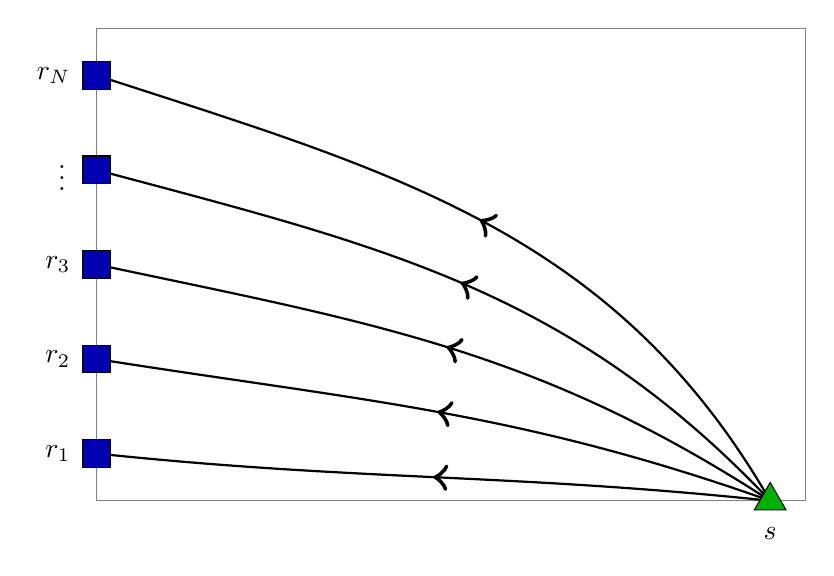
\begin{tikzpicture}[scale=1.5]
		\coordinate (tl) at (-3, 2);
		\coordinate (tr) at (3, 2);
		\coordinate (bl) at (-3, -2);
		\coordinate (br) at (3, -2);
		\coordinate (cc) at (0,0);
		\coordinate (tc) at (0,2);
		\coordinate (bc) at (0,-2);
		\coordinate (cl) at (-3, 0);
		\coordinate (cr) at (3,0);
		\coordinate (source) at ($(bl)!0.95!(br)$);
		\coordinate (receiver) at ($(bl)!0.9!(tl)$);
		\draw[gray,fill=none] (tl) rectangle (br);
		\foreach \x/\val in {0.8/$r_1$, 0.6/$r_2$, 0.4/$r_3$, 0.2/$\vdots\,$, 0/$r_N$}
		{
			\pgfmathparse{\x+0.2} \let\y=\pgfmathresult 
			\coordinate (pl) at ($(tl)!\y!(bl)$); %Point-left
			\coordinate (ppl) at ($(tl)!\x!(bl)$);
			\coordinate (ps) at ($(pl)!0.5!(ppl)$);
			\pgfmathparse{(0.8-\x)*-12/0.8 -6} \let\oang=\pgfmathresult
			\pgfmathparse{(0.8-\x)*-54/0.8 + 174} \let\iang=\pgfmathresult
			\draw [->-,thick] (source) to[out=\iang,in=\oang] (ps);
			\node[square,fill=blue!70!black] () at (ps) {};
			\node[left=6pt of ps] () {\val};
		}
		\node[triangle,fill=green!70!black] () at (source) {};
		\node[below=6pt of source] () {$s$};
		
	\end{tikzpicture}
	\caption{Wave paths on heterogeneous and continuously variable environment. The green triangle represents a source, and the blue squares each of the $N$ receivers.}
	\label{fig:sec2:wavepaths_heterogeneous-variable_environment:fig1}
\end{figure}

We now consider that each receiver represents a region in the medium (in this case, a layer), with the receiver being positioned at the center of its layer; and model the system such that each stratum has a constant speed. This will result in \cref{fig:sec2:wavepaths_heterogeneous-variable_environment:fig2}, where the wave now discontinuously changes direction and speed when changing media; however, its wavepath is continuous. The different layers are represented by the different shades of gray.

\begin{figure}[H]
	\centering
	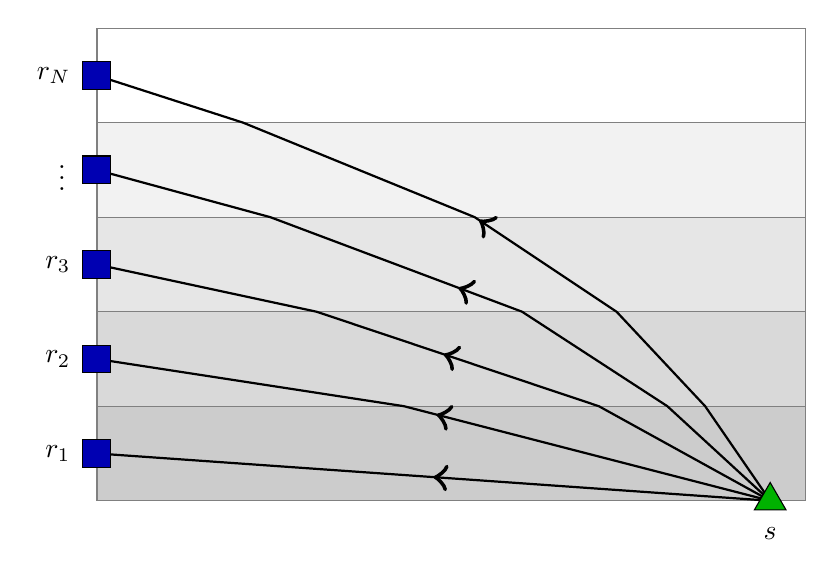
\begin{tikzpicture}[scale=1.5]
		\coordinate (tl) at (-3, 2);
		\coordinate (tr) at (3, 2);
		\coordinate (bl) at (-3, -2);
		\coordinate (br) at (3, -2);
		\coordinate (cc) at (0,0);
		\coordinate (tc) at (0,2);
		\coordinate (bc) at (0,-2);
		\coordinate (cl) at (-3, 0);
		\coordinate (cr) at (3,0);
		\coordinate (source) at ($(bl)!0.95!(br)$);
		\coordinate (receiver) at ($(bl)!0.9!(tl)$);
		\draw[gray,fill=none] (tl) rectangle (br);
		\foreach \x in {0.8,0.6,0.4,0.2,0}
		{
			\coordinate (pr) at ($(tr)!\x!(br)$); % Point-right
			\pgfmathparse{\x+0.2} \let\y=\pgfmathresult 
			\coordinate (pl) at ($(tl)!\y!(bl)$); %Point-left
			\pgfmathparse{\x * 50} \let\y=\pgfmathresult % Color calculation
			\draw[gray,very thin,fill=gray!\y!white] (pl) rectangle (pr);
		}
		\draw [->-,thick] (source) to (-3.0,-1.6);
		%
		\draw [->-,thick] (source) to (-0.4,-1.2) to (-3.0,-0.8);
		%
		\draw [->-,thick] (source) to (+1.25,-1.2) to (-1.14,-0.4) to (-3.0,0.0);
		%		
		\draw [->-,thick] (source) to (+1.83,-1.2) to (0.6,-0.4) to (-1.53,0.4) to (-3.0,0.8);
		%		
		\draw [->-,thick] (source) to (+2.15,-1.2) to (1.4,-0.4) to (0.2,0.4) to (-1.76,1.2) to (-3.0,1.6);
		%
		\foreach \x/\val in {0.8/$r_1$, 0.6/$r_2$, 0.4/$r_3$, 0.2/$\vdots\,$, 0/$r_N$}
		{
			\pgfmathparse{\x+0.2} \let\y=\pgfmathresult 
			\coordinate (pl) at ($(tl)!\y!(bl)$); %Point-left
			\coordinate (ppl) at ($(tl)!\x!(bl)$);
			\coordinate (ps) at ($(pl)!0.5!(ppl)$);
			\node[square,fill=blue!70!black] () at (ps) {};
			\node[left=6pt of ps] () {\val};
		}
		\node[triangle,fill=green!70!black] () at (source) {};
		\node[below=6pt of source] () {$s$};
		
	\end{tikzpicture}
	\caption{Wave paths on heterogeneous and discretized environment.}
	\label{fig:sec2:wavepaths_heterogeneous-variable_environment:fig2}
\end{figure}

\subsubsection{First layer}
The speed on the bottom-most layer can be trivially calculated. With the precise position of all sensors as well as for the source, 
\begin{equation}
	c_1 = \frac{d_1}{t_1},
\end{equation}
where $c_1$ is the speed on that layer; $d_1$ is the distance between the source and the first receiver; and $t_1$ is the travel time between those two points.

\subsubsection{Second layer}
Considering now the next layer and the wave that hits its respective sensor, we have the following scheme (with the $\y$-axis scaled, for clarity):

\begin{figure}[H]
	\centering
	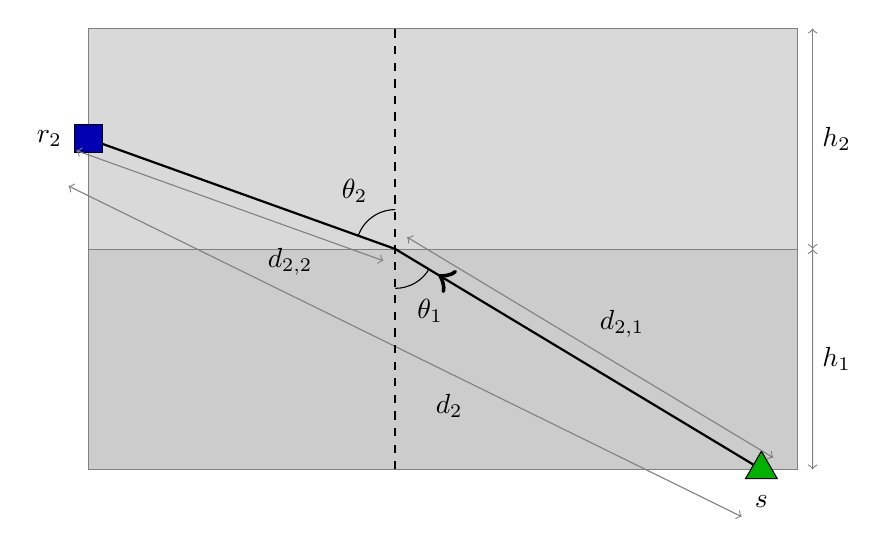
\begin{tikzpicture}[x=1.5cm,y=3.5cm]
		\coordinate (tl) at (-3, 2);
		\coordinate (tr) at (3, 2);
		\coordinate (bl) at (-3, -2);
		\coordinate (br) at (3, -2);
		\coordinate (cc) at (0,0);
		\coordinate (tc) at (0,6);
		\coordinate (bc) at (0,-2);
		\coordinate (cl) at (-3, 0);
		\coordinate (cr) at (3,0);
		%
		\coordinate (source) at ($(bl)!0.95!(br)$);
		\coordinate (r1) at ($(bl)!0.1!(tl)$);
		\coordinate (r2) at ($(bl)!0.3!(tl)$);
		%
		\coordinate (p0) at ($(tr)!0.6!(br)$);
		\coordinate (p1) at ($(tr)!0.8!(br)$);
		\coordinate (ti) at (-0.4,-0.4); % top interface
		\coordinate (bi) at (-0.4,-2); % bottom interface
		\coordinate (ci) at (-0.4,-1.2); % center interface
		%
		\draw[gray,fill=none] ($(tl)!0.6!(bl)$) rectangle (br);
		%% Draw colored rectangles
		\foreach \x in {0.8, 0.6}
		{
			\coordinate (pr) at ($(tr)!\x!(br)$); % Point-right
			\pgfmathparse{\x+0.2} \let\y=\pgfmathresult 
			\coordinate (pl) at ($(tl)!\y!(bl)$); %Point-left
			\pgfmathparse{\x * 50} \let\y=\pgfmathresult % Color calculation
			\draw[gray,very thin,fill=gray!\y!white] (pl) rectangle (pr);
		}
		%% Draw wave paths
		%		\draw [->-,thick] (source) to (r1);
		%
		\draw [->-,thick] (source) to (ci) to (r2);
		%% Draw receivers and sources
		\node[square,fill=blue!70!black] () at (r2) {};
		\node[left=6pt of r2] () {$r_2$};
		%
		\node[triangle,fill=green!70!black] () at (source) {};
		\node[below=6pt of source] () {$s$};
		%% Draw distances
		\draw[<->,thin,gray]
		([xshift=0.2cm]p1) -- ([xshift=0.2cm]br) node[pos=0.5,anchor=west,black] {$h_1$};
		%
		\draw[<->,thin,gray]
		([xshift=0.2cm]p0) -- ([xshift=0.2cm]p1) node[pos=0.5,anchor=west,black] {$h_2$};
		%
		\draw[<->,thin,gray]
		([xshift=0.15cm,yshift=0.15cm]ci) -- ([xshift=0.15cm,,yshift=0.15cm]source)
		node[pos=0.5,anchor=south west,black] {$d_{2,1}$};		
		%
		\draw[<->,thin,gray]
		([xshift=-0.15cm,yshift=-0.15cm]ci) -- ([xshift=-0.15cm,,yshift=-0.15cm]r2)
		node[pos=0.2,anchor=north east,black] {$d_{2,2}$};		
		%
		\draw[<->,thin,gray] ([xshift=-0.25cm,yshift=-0.6cm]source) -- ([xshift=-0.25cm,yshift=-0.6cm]r2) node[pos=0.4, anchor=north east,black] {$d_{2}$};
		%% Draw angles
		\draw[dashed, semithick]  (bi) -- (ti);
		\draw pic[draw,angle radius=0.5cm, "$\theta_1$", angle eccentricity=1.8] {angle=bi--ci--source};
		%
		\draw pic[draw,angle radius=0.5cm, "$\theta_2$", angle eccentricity=1.8] {angle=ti--ci--r2};
		
	\end{tikzpicture}
	\caption{Wave path in a heterogeneous and discrete environment, for the second receiver.}
	\label{fig:sec2:wavepaths_heterogeneous-variable_environment:fig3}
\end{figure}

From Snell's law, we have that
\begin{equation}
	\frac{c_1}{c_2} = \frac{\sin \theta_1}{\sin \theta_2},
\end{equation}
where $\theta_n$ is the wave's direction-of-travel's angle -- which will be called wavepath's angle -- w.r.t. the vector normal to the separation between the layers. This leads to
\begin{equation}
	c_2 = \frac{c_1 \sin \theta_2}{\sin \theta_1}
\end{equation}

The travel time for the wave that hits the second sensor will be
\begin{equation}
	t_2 = \frac{d_{2,1}}{c_1} + \frac{d_{2,2}}{c_2},
\end{equation}
in which $d_{2,1}$ is the distance traveled by the wave arriving at the second sensor, while in the first (bottom-most) layer; and $d_{2,2}$ is the distance traveled while in the second layer.

Geometrically, we also have that
\begin{equation}
	\begin{split}
		h_1
		& = \cos\theta_1 d_{2,1} \\
		& = \Sqrt{1-\sin^2\theta_1} d_{2,1}
	\end{split},
\end{equation}
\begin{equation}
	\frac{h_2}{2} = \Sqrt{1-\frac{c_2^2}{c_1^2}\sin^2\theta_1}d_{2,2}\,,
\end{equation}
where $h_1$ and $h_2$ are the heights of each receiver's layers. Defining $\sigma_1 = \sin\theta_1$, we then have
\begin{equation}
	t_2 = \frac{h_1}{c_1 \Sqrt{1-\sigma_1^2}} + \frac{h_2}{2c_2\Sqrt{1-\frac{c_2^2}{c_1^2} \sigma_1^2}}.
	\label{eq:sec3:ttt:travel-time_t2}
\end{equation}

Letting $\tau_1 = \tan \theta_1$, geometrically we have that
\begin{equation}
	d_2^2 = \pts{h_1\tau_1 + \frac{h_2}{2}\tau_2}^2 + \pts{h_1 + \frac{h_2}{2}}^2,
\end{equation}
which, via Snell's law, and trigonometrical properties, become
\begin{equation}
	d_2^2 = \pts{h_1 \frac{\sigma_1}{\Sqrt{1-\sigma_1^2}} + \frac{h_2}{2} \frac{\frac{c_2}{c_1}\sigma_1}{\Sqrt{1 - \frac{c_2^2}{c_1^2} \sigma_1^2}} }^2 + \pts{h_1 + \frac{h_2}{2}}^2,
	\label{eq:sec3:ttt:distance_d2}
\end{equation}
with $d_2$ being the distance between the source and the second (second bottom-most) receiver.

Given that $h_1$, $h_2$, $t_2$, $c_1$ and $d_2$ are known values, this results in a system with two non-linear equations \cref{eq:sec3:ttt:distance_d2,eq:sec3:ttt:travel-time_t2}, and two unknowns $\sigma_1$ and $c_2$. Solving this system leads to the knowledge of $c_2$.

%To find this solution, the Newton-Raphson method can be used. Let $f(\bvs)$ and $g(\bvs)$ be defined as
%\begin{gather*}
%	f(\bvs) = \pts{h_1 \frac{\sigma}{\Sqrt{1-\sigma^2}} + \frac{h_2}{2} \frac{\frac{c}{c_1}\sigma}{\Sqrt{1 - \frac{c^2}{c_1^2} \sigma^2}} }^2 + \pts{h_1 + \frac{h_2}{2}}^2 - d_2^2 \\
%	g(\bvs) = \frac{h_1}{c_1 \Sqrt{1-\sigma^2}} + \frac{h_2}{2c\Sqrt{1-\frac{c^2}{c_1^2} \sigma^2}} - t_2
%\end{gather*}
%with $\bvs = \tr{[c,~\sigma]}$; $c$ representing the velocity in the second layer, and $\sigma$ the emission angle of the wave ray that hits the second sensor. We define $\opt{\bvs}$ as the zero of this system of equations, in which $f(\opt{\bvs}) = g(\opt{\bvs}) = 0$.
%
%Let $F(\bvs)$ be a vector of the two previous functions, and $J(\bvs)$ its Jacobian, both given by
%\begin{gather*}
%	F(\bvs) = \begin{bmatrix}
	%		f \\
	%		g
	%	\end{bmatrix} (\bvs)\\
%	J(\bvs) = \begin{bmatrix}
	%		\pdv{f}{c} & \pdv{f}{\sigma} \\
	%		\pdv{g}{c} & \pdv{g}{\sigma}
	%	\end{bmatrix}(\bvs)
%\end{gather*}
%
%With this, and with an initial guess $\bvs{0}$, we define the iterative process
%\begin{equation}
%	\bvs{k+1} = \bvs{k} - \inv{J(\bvs)} \ast F(\bvs)
%\end{equation}
%through which we can achieve arbitrary precision; that is, we can iteratively approach $\opt{\bvs}$, leading to an arbitrarily small $F(\bvs{k+1})$.

\subsubsection{Generic layer}

We now consider the $m$-th layer, and assume that all $m-1$ previous layers were solved, knowing the velocities $c_1$ through $c_{m-1}$.

Considering the $m$-th layer, we have that
\begin{equation}
	t_m = \frac{h_m}{2c_m\Sqrt{1-\frac{c_m^2}{c_1^2}\sigma_{m,1}^2}} + \sum_{i=1}^{m-1} \frac{h_i}{c_i\Sqrt{1-\frac{c_i^2}{c_1^2}\sigma_{m,1}^2}}
	\label{eq:sec3:ttt:travel-time_mth-layer}
\end{equation}
and
\begin{equation}
	d_m^2 = \pts{\frac{h_m}{2} \frac{\frac{c_m}{c_1}\sigma_{m,1}}{\Sqrt{1-\frac{c_m^2}{c_1^2}\sigma_{m,1}^2 }} + \sum_{i=1}^{m-1} h_i \frac{\frac{c_i}{c_1}\sigma_{m,1}}{\Sqrt{1-\frac{c_i^2}{c_1^2}\sigma_{m,1}^2 }} }^2 + \pts{\frac{h_m}{2} + \sum_{i=1}^{m-1} h_m}^2.
	\label{eq:sec3:ttt:distance_mth-layer}
\end{equation}

This leads to a system with two non-linear equations \cref{eq:sec3:ttt:travel-time_mth-layer,eq:sec3:ttt:distance_mth-layer}, and two unknowns $c_m$ and $\sigma_{m,1}$; where $\sigma_{m,1} = \sin\theta_{m,1}$ is the $m$-th sensor's wavepath direction w.r.t. the normal, in the first layer. This can be solved in an identical way as for the second layer case, using the appropriate functions and variables.

Note that, although the previous $m-1$ layers' velocities are necessary to solve the $m$-th one, this process can be sped by doing the iterative search simultaneously for all velocities. That is, instead of achieving a sufficiently precise velocity for $c_2$, then $c_3$, repeating until $c_m$ is found, the iteration for all velocities can be done in the same loop, and the search for one only stop if all previous velocities have achieved sufficient precision.

%\subsubsection{Noisy measurements}
%
%We now assume that there is imprecision in our measurements, for both devices' position, and travel time. This could be caused by the devices' movements (either sources or receivers), synchronization mismatches between the devices, and unknown interactions (reflections, refractions, etc) between the waves and the environment.

%\section{Interpolation method}
%
%In this technique, we assume that the body of water follows a polynomial curve along the column of water. Similarly to the discrete method, here we assume that the speed is constant horizontally, and varies vertically. However, now we take the speed to continuously change with the height, instead of discretely.
%
%Assuming 

\subsection{Continuous fitting}

Consider any point $\bvp$ along the curve $\bvr[v]$. According to Snell's law, it will follow the equation
\begin{equation}
	\frac{\sigma(\bvp)}{c(\bvp)} = \frac{\sigma_s}{c_s},
\end{equation}
where $\sigma_s$ and $c_s$ are the (sine of) the angle of the wavepath at the source, and $c_s$ is the wave speed at the source.

Assuming that $\bvp$ is on the curve $\bvr[v]$ and is a function of time $t$, its derivative (that is, the variation of its position along $\bvr[v]$ over time) will be given by
\begin{equation}
	\dv{\bvp}{t} = [c_{\x},~c_{\y}],
\end{equation}
with $c_{\x}$ and $c_{\y}$ being the components of the wave's speed along each direction. Geometrically, this can be rewritten as
\begin{equation}
	\dv{\bvp}{t} = [c(\bvp) \sigma(\bvp),~c(\bvp) \gamma(\bvp)],
\end{equation}
where $\gamma(\bvp) = \Sqrt{1-\sigma^2(\bvp)}$, or the cosine of the angle of the wave's direction at $bvp[v]$. Through Snell's law, we then have that
\begin{equation}
	\dv{\bvp}{t} = \bts{\frac{\sigma_s}{c_s}c^2(\bvp),~c(\bvp)\Sqrt{1-\frac{\sigma_s^2}{c_s^2}c^2(\bvp)}}.
\end{equation}

This forms a system of non-linear differential equations. Given the velocity profile $c(\bvx)$ (where $\bvx$ represents a position generically in the body of water), and initial point -- the source -- $\bvp{s}$ with velocity $c_s$ and angle $\theta_s$, it is possible to determine the path traced by this wave. This is the direct problem, to determine the path given the SSP.

Meanwhile, in the inversion problem at hand there is a source, a set of arrival points $r_1$ through $r_N$ with travel-time measurements $t_1$ through $t_N$, and the objective is reconstructing the SSP $c(\bvx)$.

\subsubsection{Polynomial fitting}

The simplest solution for this problem is through a polynomial fitting. Having $N$ travel-time measurements, an $(N-1)$-degree polynomial can be fitted along these points.

We assume that $c(\bvp) \equiv c(y)$ is constant in the $\x$-axis, varying only on the $\y$-axis. It can then be written as
\begin{equation}
	c(y) = \sum_{n=0}^{N-1} a_n y^n.
\end{equation}

Writing $\bvp(t) = [p_x(t),~p_y(t)]$, then
\begin{gather}
	\dv{p_x}{t} = \frac{\sigma_s}{c_s} c^2\pts{p_y} \\
	\dv{p_y}{t} = c\pts{p_y} \Sqrt{1-\frac{\sigma_s^2}{c_s^2}c^2\pts{p_y}}.
\end{gather}

%Assuming that the right hand-side of the equations are constants w.r.t. time -- that is, assuming that the SSP $v(y)$ is constant over time, then
%\begin{gather}
%	p_x(t) = \pts{\frac{\sigma_0}{c_0} v^2(y)} t + p_{x;0} \\
%	p_y(t) = \frac{\sigma_0}{c_0} v(y) \Sqrt{1-\frac{\sigma_0^2}{c_0^2}v^2(y)} t + p_{y;0}
%\end{gather}

Note that the second equation doesn't depend on $x$, being an ordinary differential equation, with the first one depending on its solution.

We let $\lambda_m = \dfrac{\sigma_{m,s}}{c_s}$ be the wavepath's angle -- at source -- of the wavepath that hits the $m$-th sensor, and $p_{y,m}(t)$ the vertical component of the wavepath that reaches the $m$-th sensor; and via separation of variables,
\begin{equation}
	\frac{\dd p_{y,m}}{c\pts{p_{y,m}}\Sqrt{1-\lambda_1^2 c^2\pts{p_{y,m}}}} = \dd t.
\end{equation}

Integrating both sides, we achieve
\begin{equation}
	\int \frac{1}{c\pts{p_{y,m}}\Sqrt{1-\lambda_1^2 c^2\pts{p_{y,m}}}} \dd p_{y,m} = t + t_0,
\end{equation}
which, even with the knowledge/assumption that $c\pts{p_{y,m}}$ is a polynomial, still doesn't necessarily have a closed-form solution.

Together with the previous equation, which states
\begin{equation}
	\dv{p_{x,m}}{t} = \lambda_1 c^2\pts{p_{y,m}},
\end{equation}
which can also be integrated, leading to
\begin{equation}
	p_{x,m} + p_0 = \int \lambda_1 c^2\pts{p_{y,m}(t)} \dd t,
\end{equation}
where $p_{y,m}(t)$ is the vertical position as a function of time. This brings another problem, that $p_{y,m}(t)$ isn't directly obtainable, given that the previous results lead to $t(p_{y,m})$; that is, the time of arrival of the wave-path, at a given height. However, from the geometry of the problem we also have that $p_{x,m}(t)$ and $p_{y,m}(t)$ are monotonously functions. Therefore, $t(p_{y,m})$ can be inverted numerically, at least within the region of space considered in the problem.

With this, we have a system with $2N$ equations ($N$ relating to the position in the $\y$-axis, and $N$ to the $\x$-axis), and $2N$ variables (the $N$ parameters that control the polynomial $c(y)$, and the $N$ wavepath angles $\theta_{m,s}$, from which $\sigma_{m,s} = \sin \theta_{m,s}$).

Therefore, a solution to the problem can be achieved numerically and iteratively, searching for the optimal parameters. Starting with initial parameters for all variables, these can be updated iteratively, until sufficient precision is achieved.

\subsubsection{Polynomial inverse fitting}

Here, instead of assuming that $c(y)$ has a polynomial behavior, we assume that $s(y) = \frac{1}{c(y)}$ -- the slowness -- is polynomial. That is,
\begin{equation}
	s(y) = \frac{1}{c(y)} = \sum_{n=0}^{N-1} b_n y^n.
	\label{eq:sec2:polynomial_slowness}
\end{equation}

With this, the previous modeling becomes
\begin{equation}
	\begin{split}
		\dd t
		& = \frac{\dd p_{y,m}}{\frac{1}{s(p_{y,m})} \Sqrt{1-\lambda_1^2\frac{1}{s^2(p_{y,m})}}}\\
		& = \frac{s^2(p_{y,m})}{\Sqrt{s^2(p_{y,m}) - \lambda_1^2}} \, \dd p_{y,m}.
	\end{split},
\end{equation}

This modeling's solving also doesn't have a closed form, and would require a numerical-iterative solution.

%\section{1-D Vertical Scenario}

In this scenario, we now assume the source and receivers to be vertically aligned, lying on the same vertical line. This simplifies the mathematical problem, as there is no horizontal travel of the wave's direct path, and therefore no refraction.

\subsection{Discrete method}

Considering the discrete method, the vertical alignment implies that $\sigma_1 = \sigma_m = 0$. In this case, the equations from \cref{subsec:sec3:discrete_method} simplify drastically to
\begin{equation}
	t_m = \frac{h_m}{2c_m} + \sum_{i=1}^{m-1} \frac{h_i}{c_i},
\end{equation}
from which we have that
\begin{equation}
	c_m = \frac{h_m}{2\pts{t_m + \sum_{i=1}^{m-1} \frac{h_i}{c_i}}}.
\end{equation}

This leads to a direct estimation of $c_m$ instead of an iterative one, allowing a straightforward solution to the problem.

%\subsubsection{Velocity interpolation}
%
%Given the velocity $c_m$ at the measured heights, it's possible to estimate a continuous $c(y)$ such that
%\begin{equation}
%	c(y_m) = c_m
%\end{equation}
%where $y_m$ is the height of the $m$-th receiver, measured from the ocean bottom/source height. Note that $y_m \neq h_m$, as $h_m$ is the \quote{vertical width} of the layer corresponding to the $m$-th receiver.
%
%%By assuming $c(y)$ as a polynomial function,

\subsection{Polynomial fitting}
Considering the verticality assumed, there is no horizontal travel, and our problem becomes
\begin{equation}
	\dv{p_{y,m}}{t} = c\pts{p_{y,m}},
\end{equation}

Through separation of variables,
\begin{equation}
	\frac{\dd p_{y,m}}{c\pts{p_{y,m}}} = \dd t,
\end{equation}
and, integrating both sides,
\begin{equation}
	\int \frac{1}{c\pts{p_{y,m}}} \dd p_{y,m} = t + t_0,
\end{equation}
which is exactly the problem at hand: the integral of the slowness over the distance, gives the time. Using the polynomial assumption, and writing $c(y)$ as a function of its roots such that
\begin{equation}
	c(y) = A_0 \cdot \prod_{m=1}^{N-1} (y - r_m),
\end{equation}
where $r_n$ are the $N$ roots of $c(y)$; we then have
\begin{equation}
	t + t_0 = \int \frac{1}{A_0 \prod_{n=1}^{N-1} (p_y-r_n)} \dd p_y .
\end{equation}

Assuming no repeated roots, through partial fractions we get
\begin{equation}
	\frac{1}{A_0 \prod_{n=1}^{N-1} (p_y-r_n)} = \sum_{n=1}^{N-1} \frac {C_n}{p_y - r_n},
\end{equation}
where
\begin{equation}
	C_j = \frac{1}{A_0} \prod_{\substack{n=1\\n\neq j}}^{N-1} \frac{1}{r_j - r_n}.
\end{equation}

Thus,
\begin{equation}
	\begin{split}t 
		& = \int_{0}^{y_m} \sum_{n=1}^{N-1} \frac{C_n}{p_y - r_n} \dd p_y \\
%		& = \sum_{n=1}^{N-1} C_n \ln\pts{y_m - r_n} \\
		& = \ln\pts{\prod_{n=1}^{N-1} \pts{y_m - r_n} ^{C_n}} - \ln\pts{\prod_{n=1}^{N-1} \pts{-r_n} ^{C_n}}.
	\end{split}
\end{equation}

Since the signal is produced at the source, and taking this to be at the origin of our system of coordinates, then $t(y_m=0) = 0$ for all $m$. Given the measurements on all $N$ sensors, along with their positions, this gives us a system with $N$ equations -- one for each measurement -- and $N$ variables (all $N-1$ roots of $c(y)$, along with $A_0$). Note that the parameters $C_n$ are strictly dependent on $r_n$ and $A_0$.

Having these roots and the $A_0$ parameter, one can reconstruct the SSP $c(y)$.

\subsection{Inverse polynomial fitting}

Again taking the verticality of the problem, implying $\lambda_1 = \lambda_m = 0$, our problem simplifies to
\begin{equation}
	s(p_{y,m}) \dd p_{y,m} = \dd t.
	\label{eq:sec3:vc_ipf:differential_equation}
\end{equation}

%We denote $D(y) = s^2(y)$, such that
%\begin{equation}
%	D(y) = \sum_{n=0}^{N-1} \sum_{\nu=0}^{N-1}  b_n b_\nu y^{n+\nu}
%	\label{eq:sec3:vc_ipf:func_D(y)}
%\end{equation}

Integrating \cref{eq:sec3:vc_ipf:differential_equation} from $0$ to $y_m$ with the polynomial slowness from \cref{eq:sec2:polynomial_slowness}, we achieve
\begin{equation}
	\sum_{n=0}^{N-1} \frac{b_n}{n+1}y_m^{n+1} = t + t_0,
	\label{eq:sec3:vc_ipf:func_t(hm)}
\end{equation}
where $y_m$ is the height of the $m$-th receiver. This is a linear problem with $N$ variables -- the $b_n$ parameters of the polynomial $s(y)$ -- and $N$ equations, one for each sensor. The contour condition that the source is at height $y=0$ and the time is emitted at $t=0$, lead to $t_0 = 0$.

We can write \cref{eq:sec3:vc_ipf:func_t(hm)} in vector form, such that
\begin{equation}
	\bvh{m} \bvb = t_m
\end{equation}
where $\bvh{m}$ is a row-vector and $\bvb$ is a column-vector,
\begin{subequations}
	\begin{gather}
		{\bvh{m}} = \begin{bmatrix}
				1 & y_m & \cdots & y_m^{N-1}
			\end{bmatrix}, \\
	{\bvb} = \tr{\begin{bmatrix}
			b_0 & b_1 & \cdots & b_{N-1}
		\end{bmatrix}}.
	\end{gather}
\end{subequations}

With this, we can write our problem in matrix form,
\begin{equation}
	\bvH \bvb = \bvt,
\end{equation}
in which $\bvH$ is the vertical stacking of the row-vectors $\bvh{m}$, and $\bvt$ is a column-vector of the times,
\begin{subequations}
	\begin{gather}
		\bvH = \tr{\begin{bmatrix}
				\tr{\bvh{1}} & \tr{\bvh{2}} & \cdots & \tr{\bvh{N}}
		\end{bmatrix}}, \\
		\bvt = \tr{\begin{bmatrix}
				t_1 & t_2 & \cdots & t_N
		\end{bmatrix}}.
	\end{gather}
\end{subequations}

This problem can be solved directly, resulting in
\begin{equation}
	\bvb = \inv{\bvH} \bvt,
\end{equation}
where $\bvb$ is the desired vector of parameters that control the fitted polynomial of $s(y)$.

\subsection{Spline interpolation}

Another possibility is to use Spline interpolation. That is, between any two measurements at $(y_m,t_m)$ and $(y_{m+1},t_{m+1})$, we fit a cubic function $q_m(y)$ with domain $[y_{m-1},y_{m})$ such that
\begin{subequations}
	\begin{gather}
		q_m(y_m) = t_m, \label{eq:sec3:spline:conditions:eq1} \\
		q_m(y_{m+1}) = t_{m+1},  \label{eq:sec3:spline:conditions:eq2} \\
		q_m'(y_m) = q_{m-1}'(y_m),  \label{eq:sec3:spline:conditions:eq3} \\
		q_m''(y_m) = q_{m-1}''(y_m),  \label{eq:sec3:spline:conditions:eq4} \\
		q_1''(0) = q_N''(t_N) = 0. \label{eq:sec3:spline:conditions:eq5}
	\end{gather}
\end{subequations}

These conditions result in $q(y)$ --  the composition of all Splines $q_m(y)$ -- being continuous (\cref{eq:sec3:spline:conditions:eq1,eq:sec3:spline:conditions:eq2}), with a continuous first (\cref{eq:sec3:spline:conditions:eq3}) and second (\cref{eq:sec3:spline:conditions:eq4}) derivatives. We also impose that $q_1''(0) = q_N''(y_N) = 0$, meaning that the second derivative at the end-points is zero.

The use of Splines, or piece-wise interpolation, is advantageous compared to a direct interpolation through the points, since interpolating $N$ points would result in a $N-1$-degree polynomial, which is prone to high-frequency oscillations due to Runge's phenomenon.

Thus, the problem has $4N$ parameters ($4$ per Spline, with $N$ Splines), an $4N$ equations ($2N$ from continuity + $2N-2$ from first- and second-derivative continuities + $2$ from end-point conditions).

%By taking that $t_0 = 0$ and $h_0 = 0$ -- that is, the origin of the time-height coordinate system is at the sensor -- we straightforwardly get $a_1 = c_1 = 0$. Using that $q_1''(t_1) = q_2''(t_1)$, we have that
%\begin{equation}
%	d_1 = \frac{c_2}{3t_1} + d_2
%\end{equation}
%and knowing that $q_1(t_1) = h_1$ leads to
%\begin{equation}
%	b_1 = \frac{h_1}{t_1} - d_1 t_1^2
%\end{equation}
%
%This allows us to manually calculate 4 parameters $[a_1,b_1,c_1,d_1]$, thus allowing us to eliminate four equations; namely, $q_1(t_0) = 0$, $q_1(t_1) = h_1$, $q_1''(t_0) = 0$ and $q_1''(t_1) = q_2''(t_1)$. With this, the problem can be defined matricially as

The problem can be therefore defined as
\begin{subequations}
	\begin{gather}
		\begin{bmatrix}
			\bvy{0} 	& \bv0 		& \bv0 		& \cdots & \bv0 		 & \bv0 		\\
			\bvy{1} 	& \bv0 		& \bv0 		& \cdots & \bv0 		 & \bv0 		\\
			\bv0 		& \bvy{1} 	& \bv0 		& \cdots & \bv0 		 & \bv0 		\\
			\bv0 		& \bvy{2} 	& \bv0 		& \cdots & \bv0 		 & \bv0 		\\
			\vdots 	& \vdots 	& \vdots 	& \ddots & \vdots 	 & \vdots 	\\
			\bv0 		& \bv0 		& \bv0 		& \cdots & \bv0		 & \bvy{N-1}\\
			\bv0 		& \bv0 		& \bv0 		& \cdots & \bv0 		 & \bvy{N}	\\[0.3cm]
			\bvy{1}' & -\bvy{2}' & \bv0 		& \cdots & \bv0 		 & \bv0		\\
			\bv0 		& \bvy{2}' 	& -\bvy{3}' & \cdots & \bv0 		 & \bv0 		\\
			\vdots 	& \vdots 	& \vdots 	& \ddots & \vdots 	 & \vdots 	\\
			\bv0 		& \bv0 		& \bv0 		& \cdots & \bvy{N-1}' & -\bvy{N}'\\[0.3cm]
			\bvy{1}''& -\bvy{2}''& \bv0 		& \cdots & \bv0 		 & \bv0		\\
			\bv0 		& \bvy{2}''	& -\bvy{3}''& \cdots & \bv0 		 & \bv0 		\\
			\vdots 	& \vdots 	& \vdots 	& \ddots & \vdots 	 & \vdots 	\\
			\bv0 		& \bv0 		& \bv0 		& \cdots & \bvy{N-1}''& \bvy{N}''\\[0.3cm]
			\bvy{0}''& \bv0		& \bv0 		& \cdots & \bv0		 & \bv0 		\\
			\bv0 		& \bv0		& \bv0 		& \cdots	& \bv0		 & \bvy{N}''
		\end{bmatrix}
		\begin{bmatrix}
			a_1 \\ b_1 \\ c_1 \\ d_1 \\ \vdots \\ a_N \\ b_N \\ c_N \\ d_N
		\end{bmatrix}
		=
		\begin{bmatrix}
			t_0 \\ t_1 \\ t_1 \\ t_2 \\ \vdots \\ t_{N-1} \\ t_{N} \\[0.3cm] 0 \\ 0 \\ \vdots \\ 0 \\[0.3cm] 0 \\ 0 \\ \vdots \\ 0 \\[0.3cm] 0 \\ 0
		\end{bmatrix}, \label{eq:sec3:spline:eq-system_matrices} \\[0.5cm]
		\bvY \bvp = \bvt, \label{eq:sec3:spline:eq-system_short}
	\end{gather}
\end{subequations}
in which $\bvY$ is a forward operator, $\bvp$ is the vector for the Splines control parameters, and $\bvt$ is observed travel-time vector. $\bvy{m}$, $\bvy{m}'$ and $\bvy{m}''$ are
\begin{subequations}
\begin{gather}
	\bvy{m} = \begin{bmatrix}
		1 & y_m & y_m^2 & y_m^3
	\end{bmatrix}, \\
	\bvy{m}' = \begin{bmatrix}
		0 & 1 & 2 y_m & 3 y_m^2
	\end{bmatrix}, \\
	\bvy{m}'' = \begin{bmatrix}
		0 & 0 & 2 & 6 y_m
	\end{bmatrix}.
\end{gather}
\end{subequations}

Here, it is readily noticeable that $\bvy{m}'$ and $\bvy{m}''$ are the first and second derivatives of $\bvy{m}$ with respect to $y_m$.

Given that the system of equations in \cref{eq:sec3:spline:eq-system_matrices,eq:sec3:spline:eq-system_short} is exactly defined, its solution -- the parameter vector $\bvp$ -- is given by
\begin{equation}
\bvp = \inv{\bvY} \bvt.
\end{equation}

This assumes that $\bvY$ is a full-rank matrix, allowing for an inverse.

This results in a function $q(y)$ which gives the time of the wave for each height $y$. The velocity over the column is therefore given by
\begin{equation}
	c(y) = \frac{1}{\dv{q}{y}},
\end{equation}
since $\dv{q}{y}$ results in the slowness, the inverse of $c(y)$. Note that, given the piece-wise behavior of $\dv{q}{y}$, its derivative will also be defined by parts; however, by the construction of $q(y)$ its first- and second-derivatives are continuous.

\subsection{Rational interpolation}

Another solution for the problem of rapid oscillations caused by high-order polynomials, is to use a rational interpolation. In this case, our interpolating function $q(y)$ is given by
\begin{equation}
	\begin{split}
		q(y) 
		& = \frac{P(y)}{Q(y)}\\
		& = \frac{a_0 + a_1 y + \cdots + a_{K-1}y^{K-1}}{b_0 + b_1 y + \cdots + b_{T} y^{T}},
	\end{split}
\end{equation}
where $K$ and $T$ are the number of parameters in the numerator and denominator of $q(y)$, and $K+T=N$. The function $q(y)$ interpolates the arrival-time for any height. Given the number of parameters, it is feasible to have that $q(y_m) = t_m$ for all receivers. We set $b_0 = 1$ without loss of generality.

Among the advantages of rational interpolation are flexibility and stability, due to being able to model more complex behavior than simple polynomials. We also have that its derivative is also a polynomial, which can be directly calculated given the parameters of $q(y)$.

However, the presence of both uncontrolled poles and zeros can cause problems. The correct choosing of $K$ and $T$ is also necessary, as different parameters will result in different interpolations. A common option is to choose $K = N//2$, and $T = N-K$ satisfying the condition for uniqueness.

For any point $(y_m,t_m)$, we want that
\begin{equation}
	q(y_m) = t_m,
\end{equation}
which easily becomes $P(y_m) - Q(y_m) t_m= 0$; this being expanded to
\begin{equation}
 \sum_{k=0}^{K-1} a_k y^k - \sum_{n=1}^{T} b_n y^n t_m = t_m.
\end{equation}

Similarly to before, this can be written in vector form,
\begin{equation}
	\bvy{m} \bvp = t_m,
\end{equation}
with
\begin{subequations}
	\begin{gather}
		\bvy{m} = \begin{bmatrix}
			1 & y_m & \cdots & y_m^{K-1} & -t_m & -t_m y_m & \cdots & -t_m y_m^T
		\end{bmatrix}, \\
		\bvp = \tr{\begin{bmatrix}
			a_0 & \cdots a_{K-1} & b_1 & \cdots & b_T
		\end{bmatrix}}.
	\end{gather}
\end{subequations}

And, now considering all $N$ sensors, we form a matricial system
\begin{equation}
	\bvY \bvp = \bvt,
\end{equation}
where $\bvY$ is the vertical stacking of all $\bvy{m}$, and $\bvt$ is a vertical vector of all measured times,
\begin{subequations}
	\begin{gather}
		\bvY = \tr{\begin{bmatrix}
				\tr{\bvy{1}} & \cdots & \tr{\bvy{N}}
		\end{bmatrix}}, \\
		\bvt = \tr{\begin{bmatrix}
				t_1 & \cdots & t_N
		\end{bmatrix}}.
	\end{gather}
\end{subequations}

The solution is given by
\begin{equation}
	\bvp = \inv{\bvY} \bvt.
\end{equation}

\subsection{Function underfitting}

Until now, we assumed no distortion and no noise in the measurements. The solutions presented also achieve no error in the measured points.

In real-life scenarios, however, we can't assume distortionless and error-free measurements. In TTT, these mismatches can be caused by movement or desyncing in the devices, thus causing errors during in the inversion procedure for estimating the SSP. Solutions also don't necessarily have to achieve zero error in the receiver points, specially considering that these measurements can have some underlying unreliability.

For this, an underfitted function could be used. In this case, for a problem with $N$ sensors, a velocity model with only $K < N$ parameters could be fitted, minimizing the error between the modeled travel-time under $c(y)$ and the measured travel-time for the $N$ sensors. A smaller $K$ would make the model more robust to errors in position and syncing, however it would also increase the model's error when compared to the measurements. Therefore, finding an appropriate $K$ would be important.

\subsubsection{Inverse polynomial underfitting}

We will take the inverse polynomial fitting approach, for which we now define that
\begin{equation}
	s(y) = \frac{1}{c(y)} = \sum_{n=0}^{K-1} b_n y^n,
\end{equation}
where we now have a summation over $K$ terms, not $N$. From this, \cref{eq:sec3:vc_ipf:func_t(hm)} becomes
\begin{equation}
	\sum_{n=0}^{K-1} \frac{b_n}{n+1} y_m^{n+1} = t_m,
\end{equation}
in which $\bar{t}_m \neq t_m$ is the estimated travel-time for the modeled slowness profile $s(y)$. The estimation error $\epsilon_m$ is therefore
\begin{equation}
	\epsilon_m = \bar{t}_m - t_m.
\end{equation}

A possible cost function is through the Mean-Squared Error (MSE), given by
\begin{equation}
	J_1(\bvb) = \sum_{m=1}^{N} \pts{\epsilon_m}^2,
\end{equation}
where $\tr{\bvb} = [b_0,b_1,\cdots,b_{K-1}]$ is a vector of the parameters that control the (under)fitting polynomial. Expanding this cost function, we obtain
\begin{equation}
	J_1(\bvb) = \sum_{m=1}^{N} \pts{\sum_{n=0}^{K-1} \frac{b_n}{n+1} y_m^{n+1} - t_m}^2 .
\end{equation}

Differentiating this w.r.t. a generic $b_u$ yields %(after considerable work, see \cref{app:appB:derivative})
\begin{equation}
	\pdv{J_1(\bvb)}{b_u} = \frac{2}{u+1} \sum_{m=1}^{N} \pts{ \sum_{n=0}^{K-1}\bts{ \frac{b_n}{n+1} y_m^{n+u+2} } - t_m y_m^{u+1} }.
\end{equation}

Setting this to $0$ (the minimum of the function) yields
\begin{equation}
	\sum_{n=0}^{K-1}\bts{ \sum_{m=1}^{N} \pts{ \frac{y_m^{n+u+2}}{n+1} } b_n } = \sum_{m=1}^{N} t_m y_m^{u+1},
\end{equation}
which can be again written in vector form,
\begin{equation}
	\bva{u} \bvb = \tau_u
\end{equation}
where
\begin{subequations}
	\begin{gather}
		\bva{u} = \begin{bmatrix}
			a_{u,0} & \cdots & a_{u,K-1}
		\end{bmatrix}, \\
		a_{u,n} = \sum_{m=1}^{N} \frac{y_m^{n+u+2}}{n+1}, \\
		\bvb = \tr{\begin{bmatrix}
				b_0 & b_1 & \cdots & b_{K-1}
		\end{bmatrix}}, \\
		\tau_u = \sum_{m=1}^{N}\frac{y_m^{n+u+2}}{n+1}.
	\end{gather}
\end{subequations}

Considering now the derivatives w.r.t. all parameters that compose $\bvb$, we have that
\begin{equation}
	\bvA \bvb = \bvtau,
\end{equation}
in which $\bvA$ is the vertical stacking of the row-vectors $\bva{u}$, and $\bvtau$ is a column-vector of the times,
\begin{subequations}
	\begin{gather}
		\bvA = \tr{\begin{bmatrix}
				\tr{\bva{0}} & \cdots & \tr{\bva{K-1}}
		\end{bmatrix}}, \\
		\bvt = \tr{\begin{bmatrix}
				t_0 & \cdots & t_{K-1}
		\end{bmatrix}}.
	\end{gather}
\end{subequations}

Now, the vector of parameters $\bvb$ can be obtained by
\begin{equation}
	\bvb = \inv{\bvA} \bvtau.
\end{equation}

Assuming $N$ equidistant points, $K = \floor{2\Sqrt{N}}$ points are sufficient for a well-conditioned function \cite{dahlquist_numerical_2008a}.

\todo{Maybe talk about Belanger fake end-points?}

%With this, our problem becomes
%\begin{equation}
%	\pdv{J_1(\bvb)}{\bvb} = \bv0
%\end{equation}
%which has $K$ equations (one for each parameter $b_u$) and $K$ variables (each $b_u$), being exactly determined and thus (generally) having a solution.
%
%Note that there is a trivial zero of $\pdv*{J_1(\bvb)}{\bvb}$ at $\bvb = \bv0$. It is easy to see that this zero doesn't correspond to a minimum (local or global), as the error isn't being minimized. However, this function is heavily non-linear, and would require an iterative process to be solved.
%
%Another possibility for the cost function is the Mean-Absolute Error (MAE), through
%\begin{equation}
%	J_2(\bvb) = \sum_{m=1}^{N} \abs{\epsilon_m}
%\end{equation}
%whose partial derivative in $b_u$ is
%\begin{equation}
%	\begin{split}
	%		\pdv{J_2(\bvb)}{b_u}
	%		& = \sum_{m=1}^{N}\sgn{\epsilon_m} \sum_{n=0}^{K-1} \frac{b_n}{n+u+1} y_m^{n+u+1} \\
	%		& = \sum_{n=0}^{K=1} \frac{b_n}{n+u+1} \sum_{m=1}^{N} \sgn{\epsilon_m} y_m^{n+u+1}
	%	\end{split}
%\end{equation}
%
%Although still non-linear, the MAE's formulation is simpler and more straightforward compared to the MSE one. This results in an easier minimization process, although leading to a different solution.

%\subsection{Function interpolation}
%
%All previously discussed methods try to estimate the velocity on each point in space. This came from the practicality in the non-vertical scenario, as there the estimation of velocity at each point in time was easier than the estimation of the position.
%
%However, under the assumption of verticality between the source and the receivers, the wavs direct path's horizontal staticity allows the determination of a 


%\subsection{Discrete-velocity interpolation}
%
%Another technique that allows for a slight mismatch between the measured travel-times at each height, and the travel-times that are produced by the model, works by interpolating between the 

\subsubsection{Rational interpolation underfitting}

\todo{Fazer rational underfitting.}

\done{Continuar {function underfitting}.}

\done{Fazer underfitting com MAE e não MSE.}

\done{Invert Spline interpolation to be t(y), not y(t).}
%
%\printbibliography
%\appendix\newpage
%\crefalias{section}{appendix}
%\crefname{appendix}{Appendix}{Appendices}
%
%\section{Inverse integration}
We assume that $x(t)$ is a monotonously increasing function From this,
%From the geometry of the problem, we also have that $p_x(t)$ and $p_y(t)$ are monotonous functions. Therefore,
\begin{figure}[H]
	\centering
	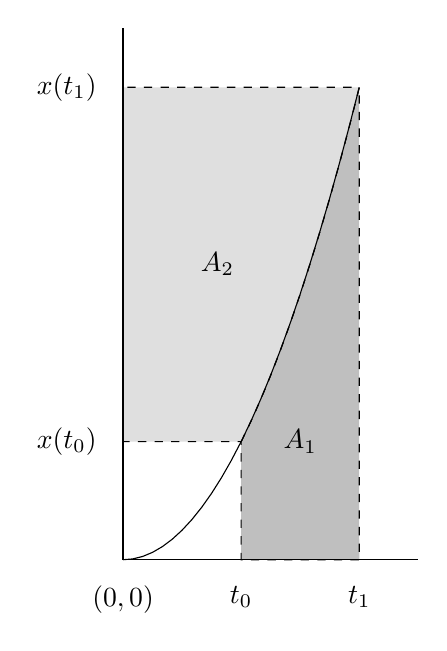
\begin{tikzpicture}[x=1.5cm,y=1.5cm]
		\filldraw [black,dashed,fill=gray!50!white,
		domain=1:2,variable=\x]
		(1,1)
		-- plot ({\x}, {\x*\x})
		-- (2,0)
		-- (1,0)
		-- cycle;
		\filldraw [black,dashed,fill=gray!25!white,
		domain=1:4,variable=\y]
		(1,1)
		-- plot ({sqrt(\y)}, {\y})
		-- (0,4)
		-- (0,1)
		-- cycle;
		\draw[domain=0:2, variable=\x]
		(0,0)
		-- plot ({\x}, {\x*\x});
		\draw (0,0) to (0,4.5);
		\draw (0,0) to (2.5,0);
		\coordinate (origin) at (0,0);
		\coordinate (t0) at (1,0);
		\coordinate (t1) at (2,0);
		\coordinate (x0) at (0,1);
		\coordinate (x1) at (0,4);
		\node[below=6pt of origin] () {$(0,0)$};
		\node[below=6pt of t0] () {$t_0$};
		\node[below=6pt of t1] () {$t_1$};
		\node[left=6pt of x0] () {$x(t_0)$};
		\node[left=6pt of x1] () {$x(t_1)$};
		\node (A1) at (1.5,1) {$A_1$};
		\node (A2) at (0.8,2.5) {$A_2$};
	\end{tikzpicture}
	\caption{Wave path in a heterogeneous and discrete environment, for the second receiver.}
	\label{}
\end{figure}

\begin{equation}
	\underbrace{\int_{t_0}^{t_1} x(t) \dd t}_{A_1} + \underbrace{\int_{x(t_0)}^{x(t_1)} \inv{x}(\tau) \dd\tau}_{A_2} + t_0 x(t_0) = t_1 x(t_1)
\end{equation}
%\section{Derivative of cost function w.r.t. polynomial coefficients}
\label{app:appB:derivative}

We have that the derivative of the cost function w.r.t. $b_u$ is
\begin{equation}
	\pdv{J_1(\bvb)}{b_u} = \sum_{m=1}^{N} \pdv{\epsilon_m^2}{b_u}
\end{equation}

Writing $\epsilon_m$ in terms of its defining integral and $t_m$, and taking its derivative w.r.t. $b_u$ results in
\begin{equation}
	\begin{split}
		\pdv{\epsilon_m^2}{b_u}
		& = \pdv{\,}{b_u} \pts{ \lint_{0}^{h_m} s^2(y,\bvb) \dd y - t_m }^2 \\
		& = \pdv{\,}{b_u} \pts{ \bts{\lint_{0}^{h_m} s^2(y,\bvb) \dd y}^2 - 2t_m\lint_{0}^{h_m} s^2(y,\bvb) \dd y + t_m^2 } \\
		& = 2\lint_{0}^{h_m}s^2(y,\bvb)\dd y \cdot \pts{ \pdv{\,}{b_u} \int_{0}^{h_m} s^2(y,\bvb) \dd y } - 2 t_m \pts{ \pdv{\,}{b_u} \int_{0}^{h_m} s^2(y,\bvb) \dd y } \\
		& = 2\int_{0}^{h_m} \pdv{s^2(y,\bvb)}{b_u} \dd y \cdot \pts{\int_{0}^{h_m} s^2(y,\bvb) \dd y - t_m}
	\end{split}
\end{equation}

From this, we need that
\begin{equation}
	\begin{split}
		\pdv{s^2(y,\bvb)}{b_u}
		& = \pdv{\,}{b_u} \pts{ \sum_{n=0}^{K-1} b_n y^n}^2 \\
		& = 2\sum_{n=0}^{K-1} b_n y^n y^u
	\end{split}
\end{equation}
which, returning to the previous equation, results in
\begin{equation}
	\begin{split}
		\pdv{\epsilon_m^2}{b_u}
		& = 4\sum_{n=0}^{K-1} \frac{b_n}{n+u+1} h_m^{n+u+1} \cdot\bts{ \sum_{\mu=0}^{K-1} \sum_{\eta=0}^{K-1} \cts{\frac{b_\mu b_\nu}{\mu+\nu+1} h_m^{\mu+\nu+1} - \frac{t_m}{(K-1)^2} } }
	\end{split}
\end{equation}

Finally, by taking the summation over all $m$ of $\pdv*{\epsilon_m^2}{b_u}$ to achieve the derivative of $J_1(\bvb)$, and noting that only the term in brackets depends on $m$, we achieve 
\begin{equation}
	\pdv{J_1(\bvb)}{b_u} = 4 \sum_{n=0}^{K-1} \frac{b_n}{n+u+1} \bts{ \sum_{\mu=0}^{K-1} \sum_{\nu=0}^{K-1} \sum_{m=1}^{N} \cts{\frac{b_\mu b_\nu }{\mu+\nu+1} h_m^{n+u+\mu+\nu+2} - \frac{t_m}{(K-1)^2}h_m^{n+u+1}} }
\end{equation}

% TODO: Add more metrics?
% TODO: Add anechoic simulation?
\end{document}

